\chapter{Texture Understanding}
\label{chapter:texturenet}
In this chapter, we discuss semantics and canonical space understanding from textured 3D surface or captured images. We discuss the semantic understanding in Section~\ref{sec:texturenet}, and the surface parameterization understanding in Section~\ref{sec:framenet}.

\section{TextureNet: Semantics from Texture}
\label{sec:texturenet}
\subsection{Introduction}
We propose a new convolutional neural network, \emph{TextureNet}~\cite{huang2018texturenet}, with a 2D convolution kernel that extracts features directly from high-resolution signals associated with 3D surface meshes.  Given a map that associates high-resolution signals with a 3D mesh surface (e.g., RGB photographic texture), we define convolutional filters that operate on those signals within domains defined by geodesic surface neighborhoods.   This approach combines the advantages of feature extraction from high-resolution signals (as in \cite{dai20183dmv}) with the advantages of view-independent convolution on 3D surface domains (as in \cite{tatarchenko2018tangent}).

During our investigation of this approach, we had to address several research issues, the most significant of which is how to define geodesic neighborhoods of a mesh.   One approach could be to compute a global UV parameterization for the entire surface and then define convolutional operators directly in UV space; however, that approach may induce significant deformations due to flattening, not always follow surface features, and/or produce seams at surface cuts.  Another approach could be to compute UV parameterizations for local neighborhoods independently; however, then adjacent neighborhoods might not be oriented consistently, reducing the ability of a network to properly learn orientation-dependent features.   Instead, we compute a 4-RoSy (four-fold rotationally symmetric) field on the surface using QuadriFlow~\cite{huang2018quadriflow} and define a new 4-RoSy convolutional operator that explicitly accounts for the 4-fold rotational ambiguity of the cross-field parameterization. A 4-RoSy (four-way rotationally symmetric) field is a configuration of 4 orthogonal tangent directions associated with each vertex in the shape of a cross that varies smoothly over the mesh surface.  Since the 4-RoSy field from QuadriFlow has no seams, aligns to shape features, induces relatively little distortion, has few singularities, and consistently orients adjacent neighborhoods (up to 4-way rotations), it provides an attractive trade-off between distortion and orientation invariance.

Results on 3D semantic segmentation benchmarks show an improvement of the 4-RoSy convolution on surfaces over alternative geometry-only approaches (by 6.4\%), plus significantly further improvement when applied to high-resolution color signals (by 6.9-8.2\% ).  With ablation studies, we verify the importance of the consistent orientation of a 4-RoSy field and demonstrate that our sampling and convolution operator works better than other alternatives.

\subsection{Related Work}
\label{related:texturenet}
\paragraph*{3D Deep Learning.}
With the availability of 3D shape databases \cite{wu20153d,chang2015shapenet,song2017semantic} and real-world labeled 3D scanning data \cite{song2015sun,armeni2017joint,dai2017scannet,chang2017matterport3d}, there is significant interest in deep learning on three-dimensional data.   Early work developed CNNs operating on 3D volumetric grids \cite{wu20153d,maturana2015voxnet}.  They have been used for 3D shape classification  \cite{qi2016volumetric,riegler2017octnet}, semantic  segmentation \cite{dai2017scannet,dai2018scancomplete}, object completion \cite{dai2017shape}, and scene completion \cite{dai2018scancomplete}.   More recently, researchers have developed methods that can take a 3D point cloud as input to a neural network and predict object classes or semantic point labels \cite{qi2017pointnet,qi2017pointnet++,tatarchenko2018tangent,su2018splatnet,atzmon2018point}.  AtlasNet~\cite{groueix2018papier} learns to generate surfaces of the 3D shape.  In our work, we utilize a sparse point sampled data representation, however, we exploit high resolution signals on geometric surface structures with a new 4-RoSy surface convolution kernel.

\paragraph*{Convolutions on Meshes.}
Several researchers have proposed methods for applying convolutional neural networks intrinsically on manifold meshes.  FeaStNet~\cite{verma2018feastnet} proposes a graph operator that establishes correspondences between filter weights. Jiang \textit{et al.}~\cite{jiang2019spherical} applies differential operators on unstructured spherical grids.
GCNN~\cite{masci2015geodesic} proposes using discrete patch operators on tangent planes parameterized by radius and angles. 
However, the orientation of their selected geodesic patches is arbitrary, and the parameterization is highly distorted or inconsistent at regions with high Gaussian curvature. 
ACNN~\cite{boscaini2016learning} observes this limitation and introduces the anisotropic heat kernels derived from principal curvatures. MoNet~\cite{monti2017geometric} further generalizes the architecture with the learnable gaussian kernels for convolutions.
The principal curvature based frame selection method is adopted by Xu \textit{et al.}~\cite{xu2017directionally} for segmentation of nonrigid surfaces, by Tatarchenko \textit{et al.}~\cite{tatarchenko2018tangent} for semantic segmentation of point clouds, and by ADD~\cite{boscaini2016anisotropic} for shape correspondence in the spectral domain. 
It naturally removes orientation ambiguity but fails to consider frame inconsistency problem, which is critical when performing feature aggregation.  Its problems are particularly pronounced in indoor scenes (which often have many planar regions where principal curvatures are undetermined) and in real-world scans (which often have noisy and uneven sampling where consistent principal curvatures are difficult to predict).   In contrast, we define a 4-RoSy field that provides consistent orientations for neighboring convolution domains.

\paragraph*{Multi-view and 2D-3D Joint Learning.}
Other researchers have investigated how to incorporate features from RGB inputs to 3D deep networks.  The typical approach is to simply assign color values to voxels, points, or mesh vertices and treat them as additional feature channels.
However, given that geometry and RGB data are at vastly different resolutions, this approach leads to significant downsampling of the color signal and thus does not take full advantage of the high-frequency patterns therein.   An alternative approach is to combine features extracted from RGB images in a multi-view CNN \cite{su2015multi}. This approach has been used for 3D semantic segmentation in 3DMV \cite{dai20183dmv}, where features are extracted from 2D RGB images and then back-projected into a 3D voxel grid where they are merged and further processed with 3D voxel convolutions.  Like our approach, 3DMV processes high-resolution RGB signals; however it convolves them in a 2D image plane, where occlusions and background clutter are confounding.  In contrast, our method directly convolves high-resolution signals intrinsically on the 3D surface which is view-independent.


\subsection{The TextureNet Approach}
Our approach performs convolutions on high-resolution signals with geodesic convolutions directly on 3D surface meshes.
The input is a 3D mesh associated with a high-resolution surface signal (e.g., a color texture map), and the outputs are learned features for a dense set of sample points that can be used for semantic segmentation and other tasks.   

Our main contribution is defining a smooth, consistently oriented domain for surface convolutions based on four-way rotationally symmetric (4-RoSy) fields.   We observe that 3D surfaces can be mapped with low-distortion to two-dimensional parameterizations anchored at dense sample points with locally consistent orientations and few singularities if we allow for a four-way ambiguity in the orientation at the sample points.   We leverage that observation in TextureNet by computing a 4-RoSy field and point sampling using QuadriFlow~\cite{huang2018quadriflow} and then building a network using new 4-RoSy convolutional filters (TextureConv) that are invariant to the four-way rotational ambiguity.   

\begin{figure}
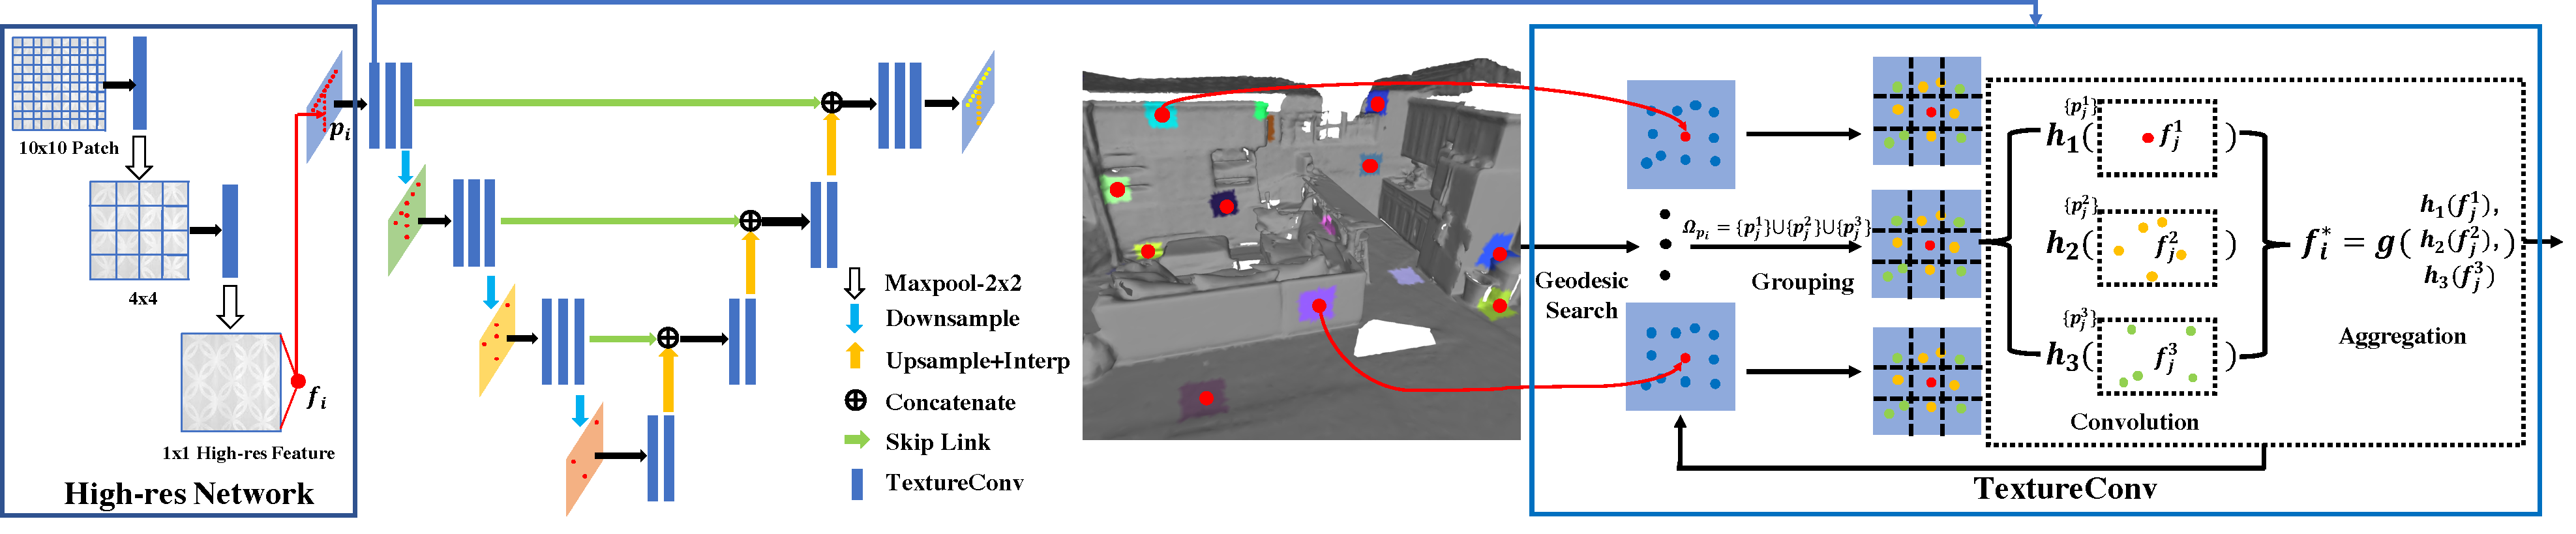
\includegraphics[width=\linewidth]{texturenet/diagram/network.pdf}
\caption{TextureNet architecture. We propose a UNet~\cite{ronneberger2015u} architecture for hierarchical feature extraction. The key innovation in the architecture is the texture convolution layer. We efficiently query the local geodesic patch for each surface point, associating each neighborhood with a local, orientation-consistent texture coordinate system. This allows us to extract the local 3D surface features as well as high-resolution signals such as associated RGB input.}
\label{fig:texturenet-approach-network}
\end{figure}

We utilize this network design to learn and extract features from high-resolution signals on surfaces by extracting surface patches with high-resolution signals oriented by the 4-RoSy field at each sample point.   The surface patches are convolved by a few TextureConv layers, pooled at sample points, and then convolved further with TextureConv layers in a UNet~\cite{ronneberger2015u} architecture, as shown in Figure~\ref{fig:texturenet-approach-network}.  For down-sampling and up-sampling, we use the furthest point sampling and three-nearest neighbor interpolation method proposed by PointNet++~\cite{qi2017pointnet++}.  The output of the network is a set of features associated with point samples that can be used for classification and other tasks.   The following sections describe the main components of the network in detail.


\subsubsection{High-Resolution Signal Representation}
\label{sec:texturenet-high-res}
Our network takes as input a high-resolution signal associated with a 3D surface mesh. In the first steps of processing, it generates a set of sample points on the mesh and defines a parameterized high-resolution patch for each sample (Section \ref{sec:texturenet-approach-param}) \jw{as follows}: For each sample point $\mathbf{p}_i$, we first compute its geodesic neighborhood $\Omega_{\rho}(\mathbf{p}_i)$ (\jw{Eq.}~\ref{eq:texturenet-omega}) with radius $\rho$. Then, we sample an NxN point cloud $\{\mathbf{q}_{xy}|-N/2\leq x,y<N/2\}$. The texture coordinates for $\mathbf{q}_{xy}$ are $((x+0.5)d,(y+0.5)d)$ -- $d$ is the distance between the adjacent pixels in the texture patch. In practice, we select $N=10$ and $d=4$mm. Finally, we use our newly proposed ``TextureConv'' and max-pooling operators (Section \ref{sec:texturenet-approach-conv}) to extract the high-res feature $\mathbf{f}_i$ for each point $\mathbf{p}_i$.  


\subsubsection{4-RoSy Surface parameterization}
\label{sec:texturenet-approach-param}
 A critical aspect of our network is to define a consistently-oriented geodesic surface parameterization for any position on a 3D mesh. Starting with some basic definitions, for a sampled point $\mathbf{p}$ on the surface, we can locally parameterize its tangent plane by two orthogonal tangent vectors $\mathbf{i}$ and $\mathbf{j}$.  Also, for any point $\mathbf{q}$ on the surface, there exists a shortest path on the surface connecting $\mathbf{p}$ and $\mathbf{q}$, e.g., the orange path in Figure~\ref{fig:texturenet-geodesic}(a). By unfolding it to the tangent plane, we can map $\mathbf{q}$ along the shortest path to $\mathbf{q^*}$.   Using these constructs, we define the local texture coordinate $\mathbf{q}$ in $\mathbf{p}$'s neighborhood as
 \begin{equation*}
     \mathbf{t}_{\mathbf{p}}(\mathbf{q}) = \begin{bmatrix}
     \mathbf{i}^T & \mathbf{j}^T
     \end{bmatrix}(\mathbf{q}^*-\mathbf{p}).
 \end{equation*}
 We additionally define the local geodesic neighborhood of $\mathbf{p}$ with receptive field $\rho$ as
\begin{equation}
\Omega_\rho(\mathbf{p}) = \{\mathbf{q}\;|\;||\mathbf{t}_{\mathbf{p}}(\mathbf{q})||_\infty < \rho\}.
\label{eq:texturenet-omega}
\end{equation}
\begin{figure}
    \centering
    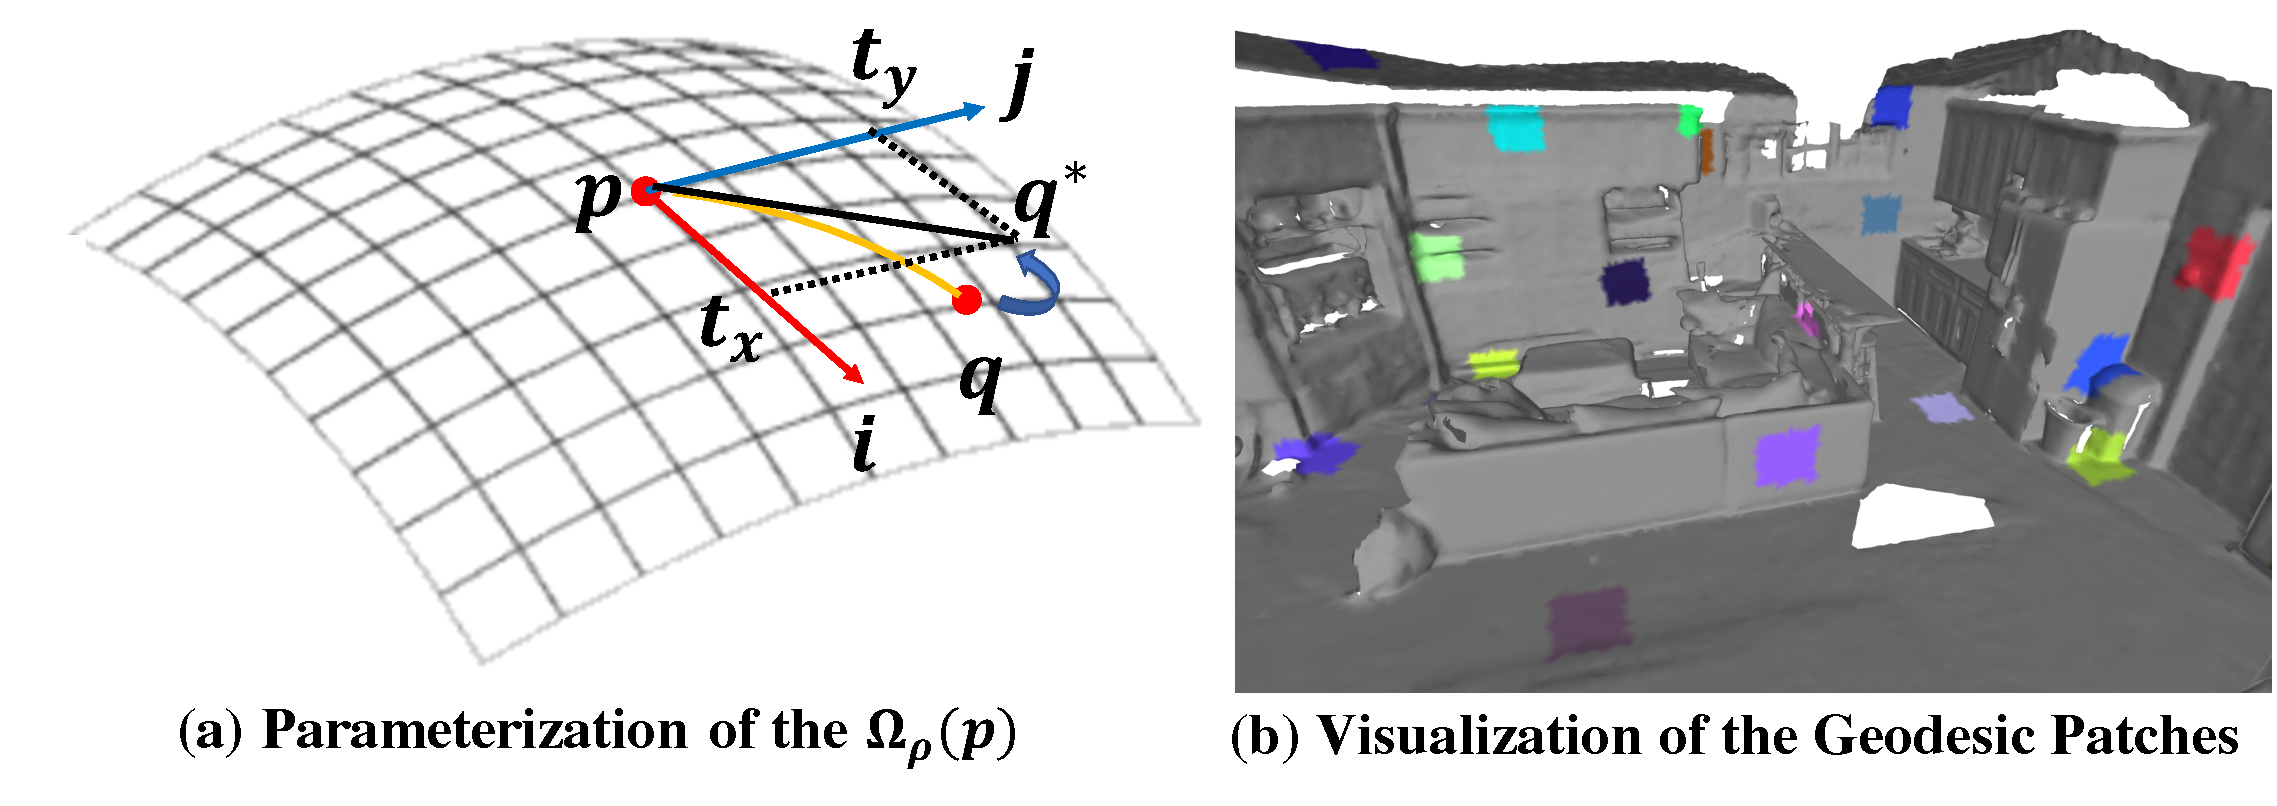
\includegraphics[width=\linewidth]{texturenet/geodesic/neighbor.pdf}
    \caption{(a) Local texture coordinates. (b) Visualization of geodesic neighborhoods $\Omega_\rho$ ($\rho$ = 20 cm) on a set of randomly sampled vertices.}
    \label{fig:texturenet-geodesic}
\end{figure}
 \begin{figure}
    \centering
     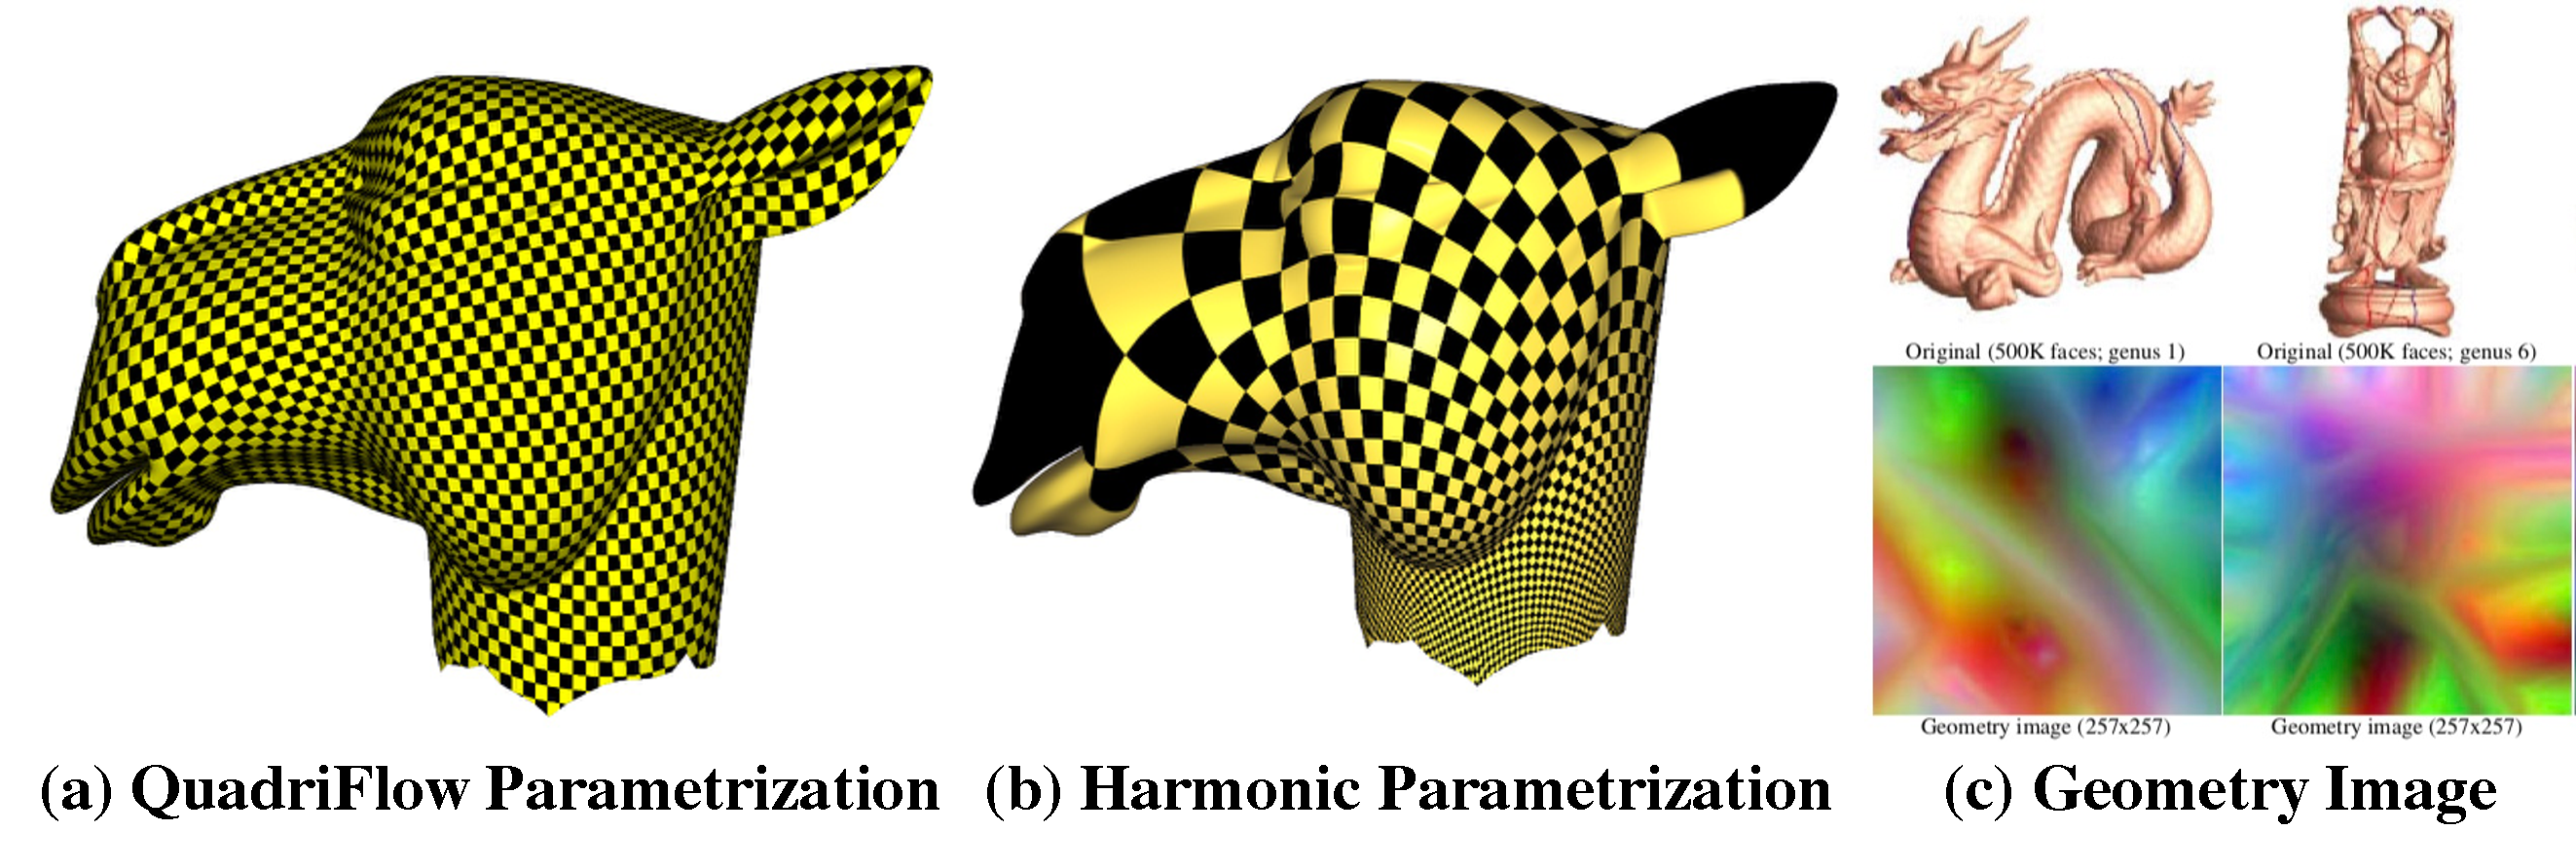
\includegraphics[width=\linewidth]{texturenet/param/param.pdf}
     \caption{(a) With an appropriate method like Quadriflow, we can get the surface parameterization aligned with shape features with negligible distortion. (b) Harmonic parameterization leads to high distortion in the scale. (c) Geometry images~\cite{gu2002geometry} result in high distortion in the orientation.}
     \label{fig:texturenet-param}
 \end{figure}
The selection for the set of mesh sampled positions $\{\mathbf{p}\}$ and their tangent vectors $\mathbf{i}$ and $\mathbf{j}$ is critical for the success of learning on a surface domain.  Ideally, we would select points whose spacing is uniform and whose tangent directions are consistently oriented at neighbors, such that the underlying parameterization has no distortions or seams, as shown in Figure~\ref{fig:texturenet-param}(a).  With those properties, we could learn convolutional operators with translation invariance exactly as we would for images.  Unfortunately, these properties are only achievable if the surface is a flat plane.   
For a general 3D surface, we can only hope to select a set of point samples and tangent vectors that minimize deviations between spacings of points and distortions of local surface parameterizations. Figure~\ref{fig:texturenet-param}(b) shows an example where harmonic surface parameterization introduces large-scale distortion -- a 2D convolution would include a large receptive field at the nose but a small one at the neck. Figure~\ref{fig:texturenet-param}(c) shows a geometry image~\cite{gu2002geometry} parameterization with high distortion in the orientation -- convolutions on such a map would have randomly distorted and irregular receptive fields, making it difficult for a network to learn canonical features.

Unfortunately, a smoothly varying direction field on the surface is usually hard to obtain. According to the study of the direction field design~\cite{ray2008n,lai2010metric}, the best-known approach to mitigate the distortion is to compute a four-way rotationally symmetric (\emph{4-RoSy}) \emph{orientation field}, which minimizes the deviation by incorporating directional ambiguity. Additionally, the orientation field needs a consistent definition among different geometries, and the most intuitive way is to make it align with the shape features like the principal curvatures. Fortunately, the extrinsic energy is used by \cite{jakob2015instant,huang2018quadriflow} to realize it. Therefore, we compute the extrinsic 4-Rosy orientation field at a uniform distribution of point samples using QuadriFlow~\cite{huang2018quadriflow} and use it to define the tangent vectors at any position on the surface. Because of the directional ambiguity, we randomly pick one direction from the cross as $\mathbf{i}$ and compute $\mathbf{j}=\mathbf{n}\times \mathbf{i}$ for any position. 

\begin{figure}
    \centering
    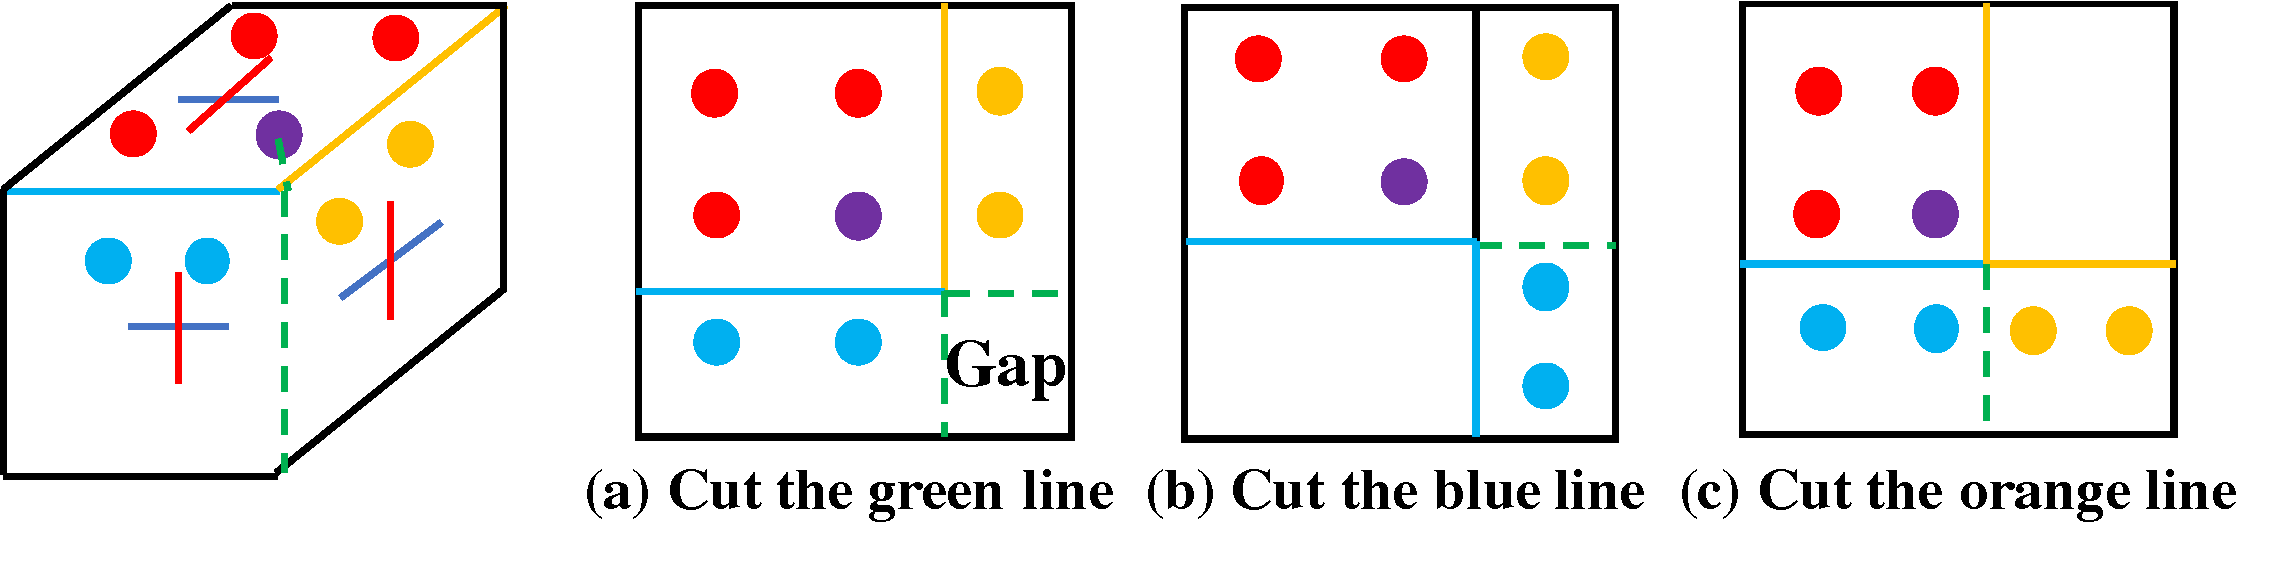
\includegraphics[width=\linewidth]{texturenet/diagram/wrap.pdf}
    \caption{Singularity at a cube vertex, (a)-(c) demonstrate three different ways of unfolding the local neighborhood. Such ambiguity is removed around the singularity by our texture coordinate definition using the shortest path. For the purple point, (a) is a valid neighborhood, while the blue points in (b) and orange points in (c) are unfolded along the paths which are not the shortest. Similarly, the ambiguity in the gap location is removed.}
    \label{fig:texturenet-wrap}
\end{figure}


Although there is a 4-way rotational ambiguity in this local parameterization of the surface (which will be addressed with a new convolutional operator in the next section), the resulting 4-RoSy field provides a way to extract geodesic neighborhoods consistently across the entire surface, even near singularities. 
Figure~\ref{fig:texturenet-wrap} (a,b,c) shows the ambiguity of possible unfolded neighborhoods at a singularity.  Since QuadriFlow~\cite{huang2018quadriflow} treats singularities as faces rather than vertices, all sampled positions have a well-defined orientation field. More importantly, the parameterization of every geodesic neighborhood is well-defined with our shortest path patch parameterization. For example, only Figure~\ref{fig:texturenet-wrap}(a) is a valid parameterization for the purple spot, while the location for the blue and orange spots in Figures~\ref{fig:texturenet-wrap}(b) and (c) are unfolded along the paths that are not the shortest. Unfolding a geodesic neighborhood around the singularity also causes another potential issue that a seam cut is usually required, leading to a gap at the 3-singularity or multiple-surface coverage at the 5-singularity. For example, there is a gap at the bottom-right corner in Figure~\ref{fig:texturenet-wrap}(a) caused by the seam cut shown as the green dot line. Fortunately, the location of the seam is also well-defined with our shortest-path definition: it must be the shortest geodesic path going through the singularity. Therefore, our definition of the local neighborhood guarantees a canonical way of surface parameterization even around corners and singularities.

\subsection{4-RoSy Surface Convolution Operator}
\label{sec:texturenet-approach-conv}
\begin{figure}
     \centering
     \begin{minipage}{0.32\linewidth}
     \centering
     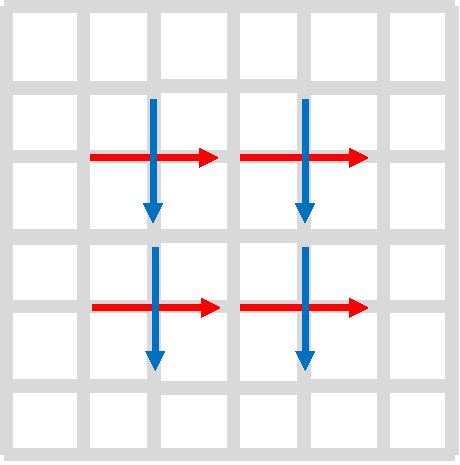
\includegraphics[width=\linewidth,height=\linewidth]{texturenet/diagram/image_coordinate.pdf}\\
     \footnotesize{
     (a) Image Coordinate
     }
     \end{minipage}
     \begin{minipage}{0.32\linewidth}
     \centering
     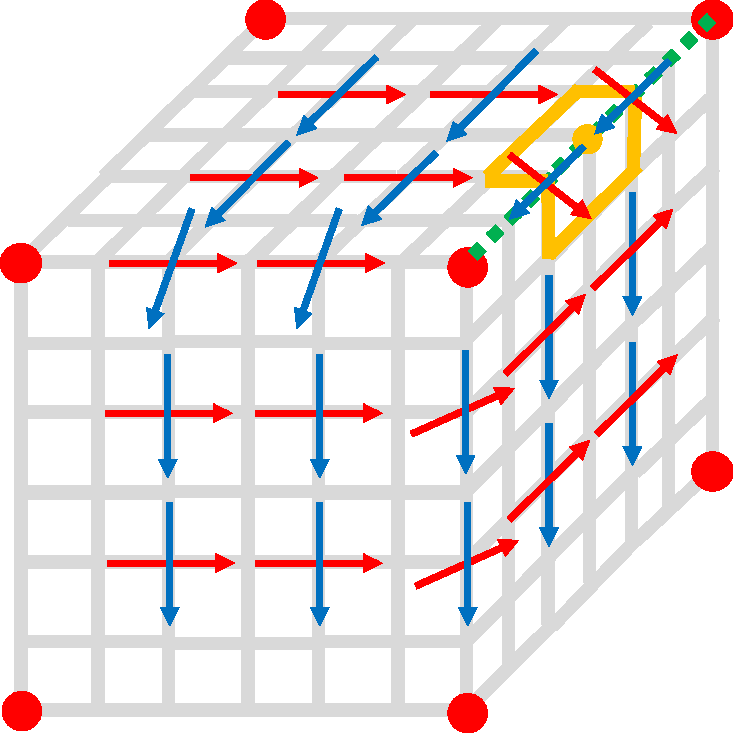
\includegraphics[width=\linewidth,height=\linewidth]{texturenet/diagram/cube_coordinate.pdf}\\
     \footnotesize{
     (b) 3D parametrization
     }
     \end{minipage}
     \begin{minipage}{0.32\linewidth}
     \centering
     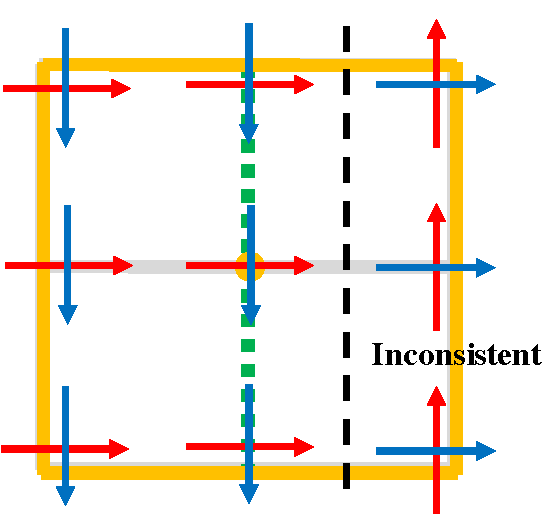
\includegraphics[width=\linewidth,height=\linewidth]{texturenet/diagram/conv_coordinate.pdf}\\
     \footnotesize{
     (c) Inconsistent Frame
     }
     \end{minipage}
     \caption{(a) Traditional convolution kernel on a regular grid. (b) Frames defined by the orientation field on a 3D cube. (c) For the patch highlighted in orange in (b), multi-layer feature aggregation would be problematic with traditional convolution due to the frame inconsistency caused by the directional ambiguity of the orientation field.}
     \label{fig:texturenet-singular}
 \end{figure}

TextureNet~is a network architecture composed of convolutional operators acting on geodesic neighborhoods of sample points with 4-RoSy parameterizations.
The input to each convolutional layer is three-fold: 1) a set of 3D sample points associated with features (e.g., RGB, normals, or features computed from high-resolution surface patches or previous layers); 2) a coordinate system stored as two tangent vectors representing the 4-RoSy cross-field for each point sample; and 3) a coarse triangle mesh, where each face is associated with the set of extracted sampled points and connectivity indices that support fast geodesic patch query and texture coordinate computation for the samples inside a geodesic neighborhood, much like the PTex~\cite{burley2008ptex} representation for textures. 

Our key contribution in this section is the design of a convolution operator suitable for 4-RoSy fields. 
The problem is that we cannot use traditional 3x3 convolution kernels on domains parameterized with 4-RoSy fields without inducing inconsistent feature aggregation at higher levels.  Figure~\ref{fig:texturenet-singular} demonstrates the problem for a simple example.  Figure~\ref{fig:texturenet-singular}(a) shows 3x3 convolution in a traditional flat domain. Figure~\ref{fig:texturenet-singular}(b) shows the frames defined by our 4-RoSy orientation field of the 3D cube where red spots represent the singularities. Although the cross-field in the orange patch is consistent under the 4-RoSy metric, the frames are not parallel when they are unfolded into a plane (Figure~\ref{fig:texturenet-singular}(c)). Aggregation of features inside such a patch is therefore problematic.

``TextureConv'' is our solution to remove the directional ambiguity. It consists of four layers (in Figure~\ref{fig:texturenet-approach-network}), including geodesic patch search, texture space grouping, convolution and aggregation. To extract the geodesic patch for each input point $\Omega_\rho(\mathbf{p})$, we use breadth-first search with the priority queue to extract the face set in the order of \jw{geodesic distance from face center to $\mathbf{p}$}. We estimate the texture coordinate at the face center as well as its local tangent coordinate system, recorded as $(\mathbf{t}_f,\mathbf{i}_f,\mathbf{j}_f)$. In order to expand the search tree from face $u$ to $v$, we can approximate the texture coordinate at the face center as $\mathbf{t}_{v} = \mathbf{t}_{u} + (\mathbf{i}_u,\mathbf{j}_u)^T (\mathbf{c}_v - \mathbf{c}_u)$, where $\mathbf{c}_f$ represents the center position of the face $f$. $\mathbf{i}_v$ and $\mathbf{j}_v$ can be computed by rotating the coordinate system around the shared edge from face $u$ to $v$. After having the face set inside the geodesic patch, we can find the sampled points set associated with these faces. We estimate the texture coordinate of every sampled point $\mathbf{q}$ associated with each face $f$ as $\mathbf{t}_\mathbf{p}(\mathbf{q})=\mathbf{t}_f+(\mathbf{i}_f,\mathbf{j}_f)^T(\mathbf{q} - \mathbf{c}_f)$. By testing $||\mathbf{t}_\mathbf{p}(\mathbf{q})||_\infty < \rho$, we can determine the sampled points inside the geodesic patch $\Omega_\rho(\mathbf{p})$.

The texture space grouping layer segments the local neighborhood into 3x3 patches in the texture space, each of which is a square with edge length as $2\rho/3$, as shown in Figure~\ref{fig:texturenet-approach-network} (after the ``grouping arrow''). We could directly borrow the image convolution method linearly transform each point feature with 9 different weights according to their belonging patch. However, we propose a 4-RoSy convolution kernel to deal with the directional ambiguity. As shown in Figure~\ref{fig:texturenet-approach-network}, all sampled points can be categorized as at the corners ($\{\mathbf{p}_j^1\}$), edges ($\{\mathbf{p}_j^2\}$) or the center ($\{\mathbf{p}_j^3\}$). Each sampled point feature is convolved with a 1x1 convolution as $h_1$, $h_2$ or $h_3$ based on its category. The extracted 4-rosy feature removes the ambiguity and allows higher-level feature aggregation. The \jw{channel-wise} aggregation operator $g$ can be max-pooling or average-pooling followed by the ReLu layer. In the task for semantic segmentation, we choose max-pooling since it is better at preserving salient signals.

\subsection{TextureNet Evaluation}

To investigate the performance of TextureNet, we ran a series of 3D semantic segmentation experiments for indoor scenes.   In all experiments, we train and test on the standard splits of the ScanNet~\cite{dai2017scannet} and Matterport3D~\cite{dai2017scannet} datasets.  Following previous works, we report mean class intersection-over-union (mIoU) results for ScanNet and mean class accuracy for Matterport3D.

%%%%%%%%%%%%%%%%%%%%%%%%%%%%%%%%%%%%%%%%%%%%
\para{Comparison to State-of-the-Art.}
\label{sec:texturenet-eval-result}

\begin{table*}
    \centering
    \scriptsize
    \tabcolsep=0.02cm
    \begin{tabular}{|c|c|c|c|c|c|c|c|c|c|c|c|c|c|c|c|c|c|c|c|c||c|}
        \hline
        Input & wall & floor & cab & bed & chair & sofa & table & door & wind & shf & pic & cntr & desk & curt & fridg & show & toil & sink & bath & other & avg\\
        \hline
        PN$^+$\cite{qi2017pointnet++} & 66.4 & 91.5 & 27.8 & 56.3 & 64.0 & 52.7 & 37.3 & 28.3 & 36.1 & 59.2 & 6.7 & 28.0 & 26.2 & 45.4 & 25.6 & 22.0 & 63.5 & 38.8 & 54.4 & 20.0 & 42.5\\
        \hline
        SplatNet\cite{su2018splatnet} & \textbf{69.9} & 92.5 & 31.1 & 51.1 & 65.6 & 51.0 & 38.3 & 19.7 & 26.7 & 60.6 & 0.0 & 24.5 & 32.8 & 40.5 & 0.0 & 24.9 & 59.3 & 27.1 & 47.2 & 22.7 & 39.3 \\
        \hline
        Tangent\cite{tatarchenko2018tangent} & 63.3 & 91.8 & 36.9 & 64.6 & 64.5 & 56.2 & 42.7 & 27.9 & 35.2 & 47.4 & 14.7 & 35.3 & 28.2 & 25.8 & 28.3 & 29.4 & 61.9 & 48.7 & 43.7 & 29.8 & 43.8\\
        \hline
        3DMV\cite{dai20183dmv} & 60.2 & 79.6 & 42.4 & 53.8 & 60.6 & 50.7 & 41.3 & 37.8 & 53.9 & 64.3 & 21.4 & 31.0 & 43.3 & 57.4 & \textbf{53.7} & 20.8 & 69.3 & 47.2 & 48.4 & 30.1 & 48.4\\
        \hline
        Ours & 68.0 & \textbf{93.5} & \textbf{49.4} & \textbf{66.4} & \textbf{71.9} & \textbf{63.6} & \textbf{46.4} & \textbf{39.6} & \textbf{56.8} & \textbf{67.1} & \textbf{22.5} & \textbf{44.5} & \textbf{41.1} & \textbf{67.8} & 41.2 & \textbf{53.5} & \textbf{79.4} & \textbf{56.5} & \textbf{67.2} & \textbf{35.6} & \textbf{56.6}\\
        \hline
    \end{tabular}\\
    (a) ScanNet (v2) (mean class IoU)
    \centering
    \tabcolsep=0.015cm
    \begin{tabular}{|c|c|c|c|c|c|c|c|c|c|c|c|c|c|c|c|c|c|c|c|c|c||c|}
        \hline
        Input & wall & floor & cab & bed & chair & sofa & table & door & wind & shf & pic & cntr & desk & curt & ceil & fridg & show & toil & sink & bath & other & avg\\
        \hline
        PN$^+$\cite{qi2017pointnet++} & 80.1 & 81.3 & 34.1 & 71.8 & 59.7 & 63.5 & \textbf{58.1} & 49.6 & 28.7 & 1.1 & 34.3 & 10.1 & 0.0 & 68.8 & 79.3 & 0.0 & 29.0 & 70.4 & 29.4 & 62.1 & 8.5 & 43.8 \\
        \hline
        SplatNet\cite{su2018splatnet} & \textbf{90.8} & \textbf{95.7} & 30.3 & 19.9 & \textbf{77.6} & 36.9 & 19.8 & 33.6 & 15.8 & 15.7 & 0.0 & 0.0 & 0.0 & 12.3 & 75.7 & 0.0 & 0.0 & 10.6 & 4.1 & 20.3 & 1.7 & 26.7 \\
        \hline
        Tangent\cite{tatarchenko2018tangent} & 56.0 & 87.7 & 41.5 & 73.6 & 60.7 & 69.3 & 38.1 & 55.0 & 30.7 & 33.9 & 50.6 & 38.5 & 19.7 & 48.0 & 45.1 & 22.6 & 35.9 & 50.7 & 49.3 & 56.4 & 16.6 & 46.8 \\
        \hline
        3DMV\cite{dai20183dmv} & 79.6 & 95.5 & \textbf{59.7} & 82.3 & 70.5 & \textbf{73.3} & 48.5 & 64.3 & 55.7 & 8.3 & 55.4 & 34.8 & 2.4 & \textbf{80.1} & \textbf{94.8} & 4.7 & 54.0 & 71.1 & 47.5 & 76.7 & 19.9 & 56.1 \\
        \hline
        Ours & 63.6 & 91.3 & 47.6 & \textbf{82.4} & 66.5 & 64.5 & 45.5 & \textbf{69.4} & \textbf{60.9} & \textbf{30.5} & \textbf{77.0} & \textbf{42.3} & \textbf{44.3} & 75.2 & 92.3 & \textbf{49.1} & \textbf{66.0} & \textbf{80.1} & \textbf{60.6} & \textbf{86.4} & \textbf{27.5} & \textbf{63.0} \\
        \hline
    \end{tabular}\\
    (b) Matterport3D (mean class accuracy)
    \caption{Comparison with the state-of-the-art methods for 3D semantic segmentation on the (a) ScanNet v2, and (b) Matterport3D~\cite{chang2017matterport3d} benchmarks. PN$^+$, SplatNet, and Tangent Convolution use points with per-point normal and color as input. 3DMV uses 2D images and voxels.  Ours uses grid points with high-res 10x10 texture patches.}
    \label{tab:texturenet-mainresult}
\end{table*}

\begin{figure*}
    \centering
    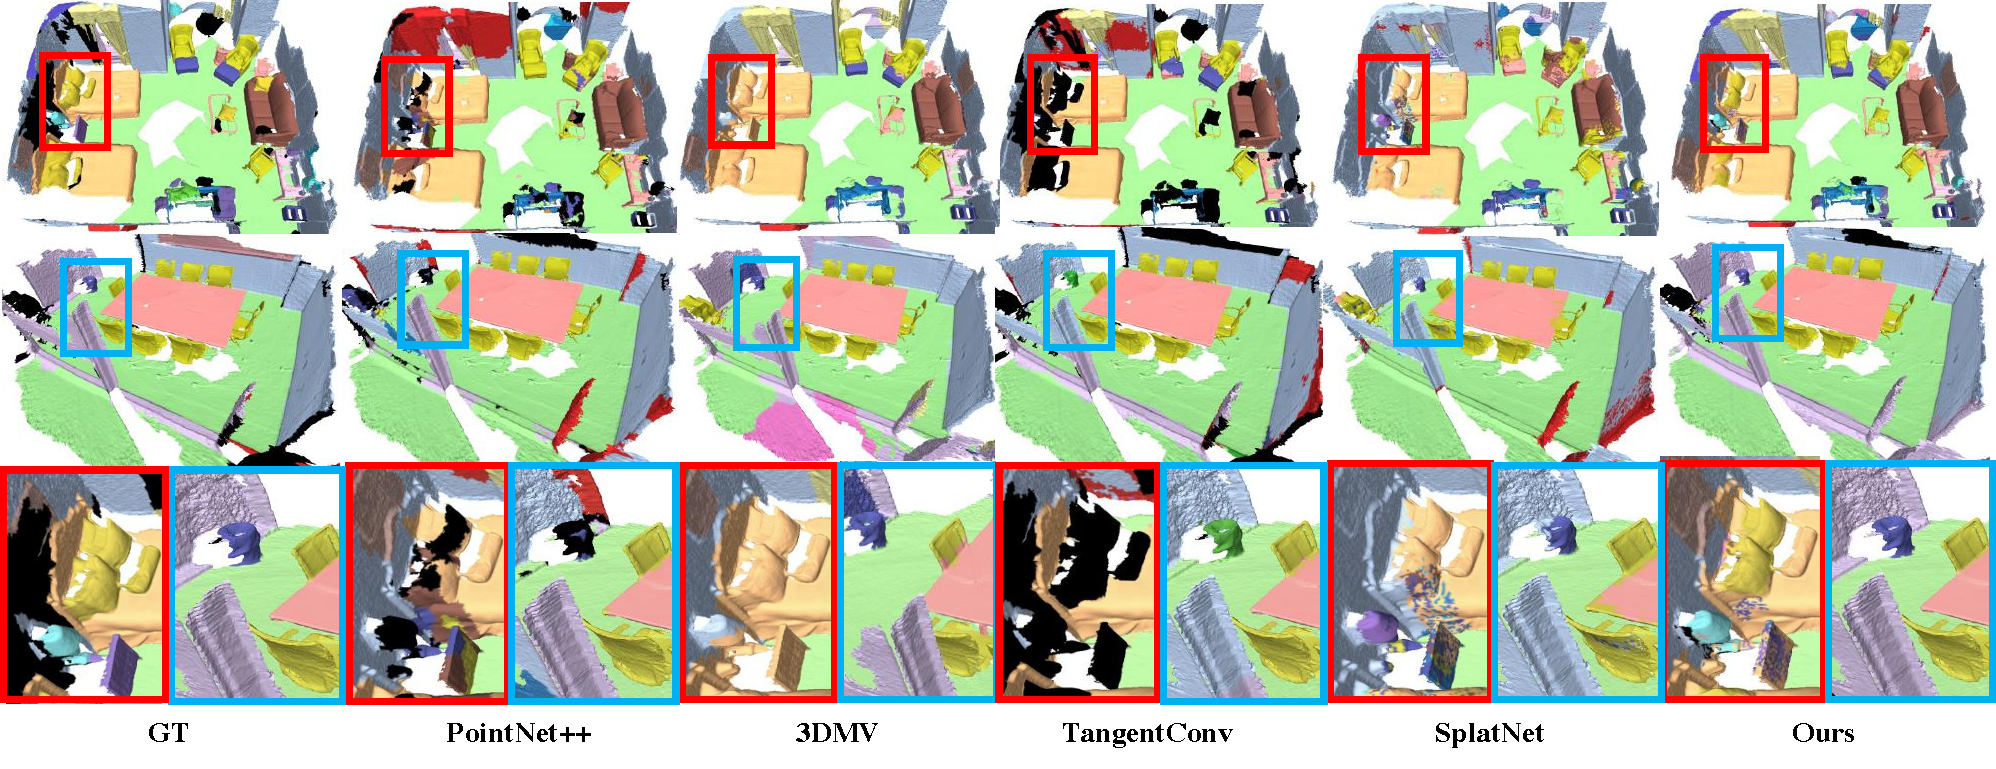
\includegraphics[width=\linewidth]{texturenet/result/scannet_horizontal.pdf}
    \caption{Visualization on ScanNet (v2)~\cite{dai2017scannet}. In the first row, we correctly predict the lamp, pillow, picture, and part of the cabinet, while other methods fail. In the second row, we predict the window and the trash bin correctly, while 3DMV~\cite{dai20183dmv} predicts part of the window as the trash bin and other methods fail.  The third row (zoom-in) highlights the differences.}
    \label{fig:texturenet-result-scannet}
\end{figure*}

\begin{figure}[t]
    \centering
    \begin{minipage}{0.32\linewidth}
    \centering
    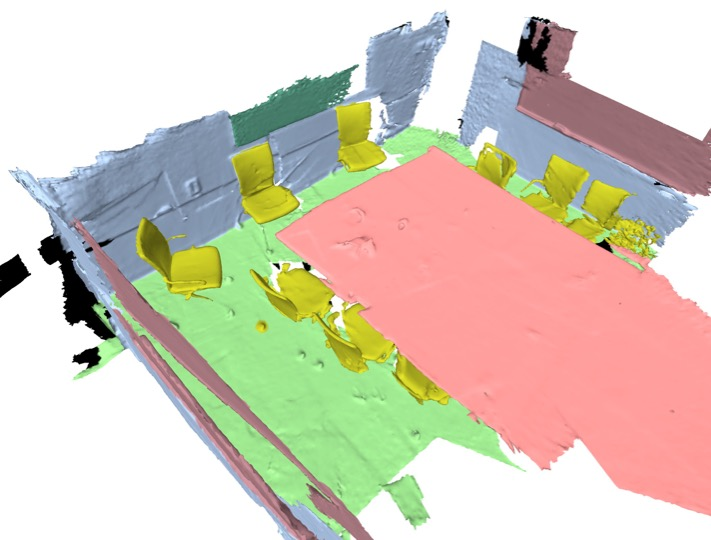
\includegraphics[width=\linewidth]{texturenet/neighbors/gt.jpg}
    (a) Ground Truth
    \end{minipage}
    \begin{minipage}{0.32\linewidth}
    \centering
    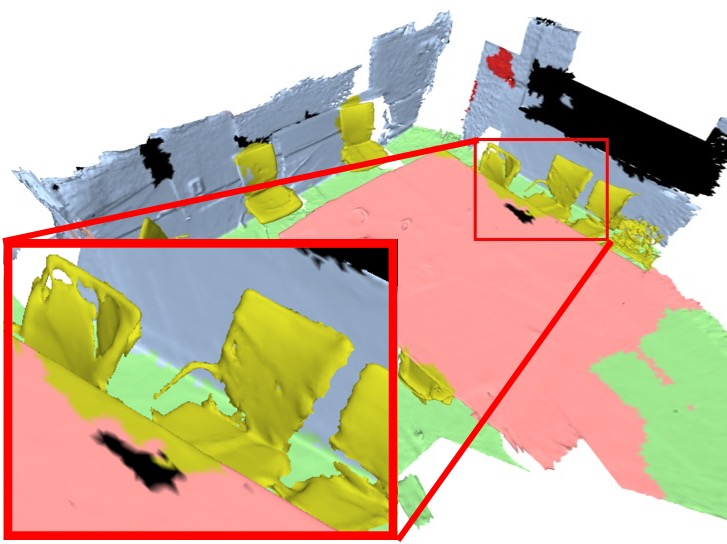
\includegraphics[width=\linewidth]{texturenet/neighbors/pointnet.jpg}
    (b) Ball
    \end{minipage}
    \begin{minipage}{0.32\linewidth}
    \centering
    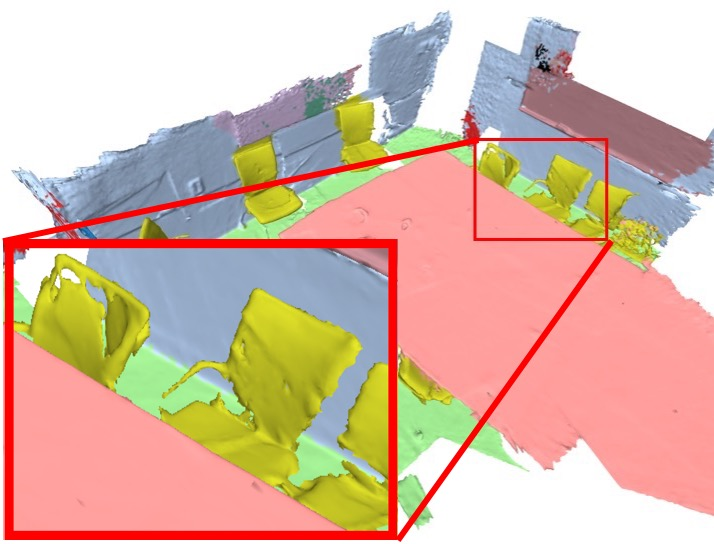
\includegraphics[width=\linewidth]{texturenet/neighbors/ours.jpg}
    (c) Ours
    \end{minipage}
    \caption{Visual results using different neighborhoods. With euclidean ball as a neighborhood, part of the table is predicted as the chair, since they belong to the same euclidean ball. This issue is solved by extracting features from the geodesic patches.}
    \label{fig:texturenet-neighbor}
\end{figure}

\begin{figure}[t]
    \centering
    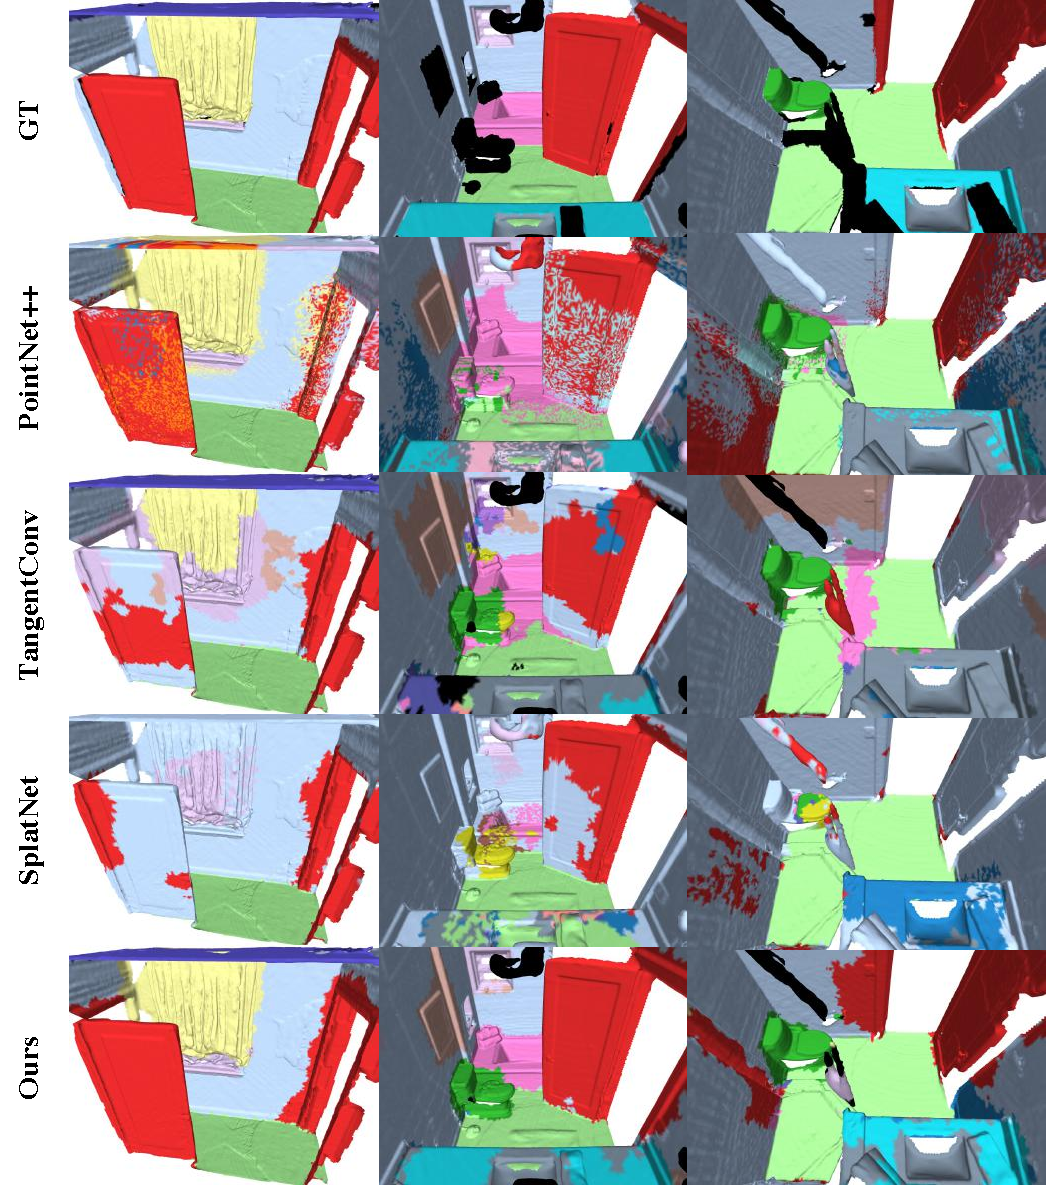
\includegraphics[width=0.75\linewidth]{texturenet/result/matterport.pdf}
    \caption{Visual results on Matterport3D~\cite{chang2017matterport3d}. In all examples, our method is better at predicting the door, the toilet, the sink, the bathtub, and the curtain.}
    \label{fig:texturenet-result-Matterport3D}
\end{figure}

Our main result is a comparison of TextureNet to state-of-the-art methods for 3D semantic segmentation.  For this experiment, all methods utilize both color and geometry in their native formats.   Specifically, PointNet++~\cite{qi2017pointnet++}, Tangent Convolution~\cite{tatarchenko2018tangent}, SplatNet~\cite{su2018splatnet} use points with per-point normals and colors; 3DMV~\cite{dai20183dmv} uses 2D image features back-projected onto voxels; and Ours uses high-res 10x10 texture patches extracted from geodesic neighborhoods at sample points.

Table~\ref{tab:texturenet-mainresult} reports the mean IoU scores for all 20 classes of the ScanNet benchmark on the ScanNet (v2) and mean class accuracy on Matterport3D datasets.   They show that TextureNet (Ours) provides the best results on 18/20 classes for Scannet and 12/20 classes for Matterport3D.  Overall, the mean class IoU for Ours is 8.2\% higher than the previous state-of-the-art (3DMV) on ScanNet (48.4\% vs. 56.6\%), and our mean class accuracy is 6.9\% higher on Matterport3D (56.1\% vs. 63.0\%).  

Qualitative visual comparisons of the results shown in Figures~\ref{fig:texturenet-result-scannet}-\ref{fig:texturenet-result-Matterport3D} suggest that the differences between methods are often where high-resolution surface patterns are discriminating (e.g., the curtain and pillows in the top row of Figure~\ref{fig:texturenet-result-scannet}) and where geodesic neighborhoods are more informative than Euclidean ones (e.g., the lamp next to the bed).  Figure~\ref{fig:texturenet-neighbor} shows a case where convolutions with the geodesic neighborhoods clearly outperform their Euclidean counterparts. In Figure~\ref{fig:texturenet-neighbor}(b), part of the table is predicted as chair, probably because it is in a Euclidean ball covering nearby chairs. This problem is solved with our method based on geodesic patch neighborhoods. As shown in Figure~\ref{fig:texturenet-neighbor}(c), the table and the chairs are clearly segmented.

%%%%%%%%%%%%%%%%%%%%%%%%%%%%%%%%%%%%%%%%%%%%
\para{Effect of 4-RoSy Surface Parameterization.}

Our second experiment is designed to test how different surface parameterizations affect semantic segmentation performance -- i.e., how does the choice of the orientation field affect the learning process?   The simplest choice is to pick an arbitrary direction on the tangent plane as the x-axis, similar to GCNN~\cite{masci2015geodesic}, (Figure~\ref{fig:texturenet-coordinate}(a)).  A second option adopted by Tangent Convolution~\cite{tatarchenko2018tangent} considers a set of points $\mathbf{q}$ in a Euclidean ball centered at $\mathbf{p}$ and parameterizes the tangent plane by two eigenvectors corresponding to the largest two eigenvalues of the covariance matrix $\sum_{q}(p-q)(p-q)^T$.  A critical problem of this formulation is that the principal directions cannot be robustly analyzed at planar regions or noisy surfaces (Figure~\ref{fig:texturenet-coordinate}(b)). It also introduces inconsistency to the coordinate systems of the neighboring points, which vexes the feature aggregation at higher levels.  A third alternative is to use the intrinsic energy function~\cite{jakob2015instant} or other widely used direction field synthesis technique~\cite{ray2008n,lai2010metric}, which is not geometry-aware and therefore variant to 3D rigid transformation (Figure~\ref{fig:texturenet-coordinate}(c)). Our choice is to use the extrinsic energy to synthesize the direction field~\cite{huang2018quadriflow,jakob2015instant}, which is globally consistent and the only variant to geometry itself (Figure~\ref{fig:texturenet-coordinate}(d)).

\begin{figure}
    \centering
    \begin{minipage}{0.24\linewidth}
    \centering
    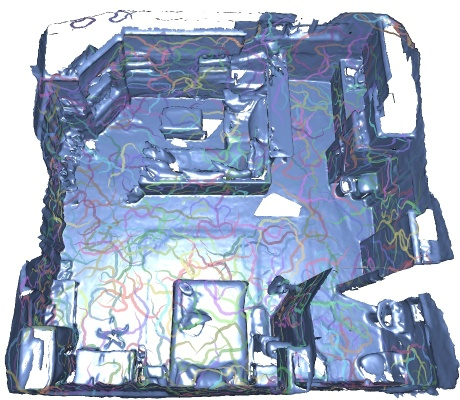
\includegraphics[width=\linewidth]{texturenet/field/random.jpg}
    (a) RandomVec
    \end{minipage}
    \begin{minipage}{0.24\linewidth}
    \centering
    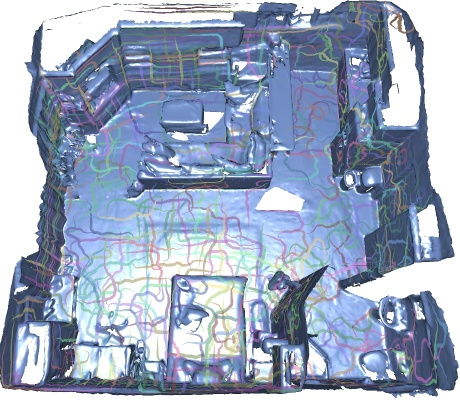
\includegraphics[width=\linewidth]{texturenet/field/eigen.jpg}
    (b) EigenVec
    \end{minipage}
    \begin{minipage}{0.24\linewidth}
    \centering
    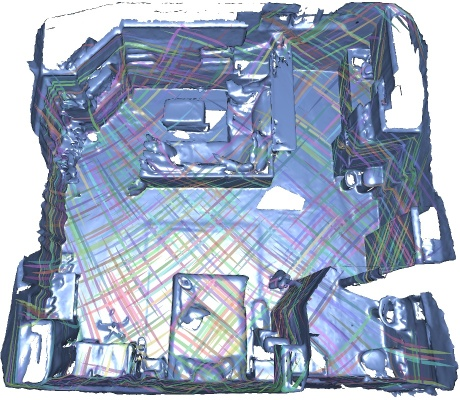
\includegraphics[width=\linewidth]{texturenet/field/intrinsic.jpg}
    (c) Intrinsic
    \end{minipage}
    \begin{minipage}{0.24\linewidth}
    \centering
    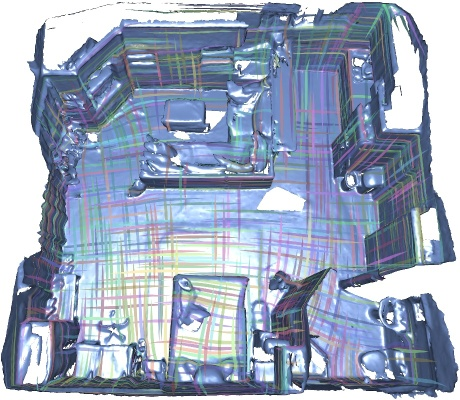
\includegraphics[width=\linewidth]{texturenet/field/extrinsic.jpg}
    (d) Extrinsic
    \end{minipage}
    \caption{Direction fields from different methods. (a) Random directions lead to inconsistent frames. (b) Eigenvectors suffer from the same issue at flat area. (c) Intrinsic-energy based orientation field does not align to the shape features. (d) Our extrinsic-based method generates consistent orientation fields aligned with surface features.}
    \label{fig:texturenet-coordinate}
\end{figure}

\begin{table*}
    \centering
    \scriptsize
    \tabcolsep=0.04cm
    \begin{tabular}{|c|c|c|c|c|c|c|c|c|c|c|c|c|c|c|c|c|c|c|c|c|c|c|}
        \hline
        Input & wall & floor & cab & bed & chair & sofa & table & door & wind & bkshf & pic & cntr & desk & curt & fridg & show & toil & sink & bath & other & ave\\
        \hline
        Random & 37.6 & \textbf{92.5} & 37.0 & 63.7 & 28.5 & 56.9 & 27.6 & 15.3 & 31.0 & 47.6 & 16.5 & 36.6 & \textbf{53.3} & \textbf{51.2} & 15.4 & 24.7 & 59.3 & 47.6 & 53.3 & 27.0 & 41.1 \\
        \hline
        Intrinsic & 47.4 & 91.9 & 35.3 & 62.5 & 55.8 & 44.8 & 37.5 & 29.8 & 40.5 & 40.9 & 16.7 & 41.5 & 39.9 & 42.1 & 20.4 & 24.3 & 85.6 & 44.5 & 58.3 & 29.5 & 44.4 \\
        \hline
        EigenVec & 45.3 & 79.0 & 32.2 & 53.4 & 59.8 & 40.4 & 32.2 & 28.8 & 40.5 & 43.4 & \textbf{17.8} & 39.5 & 32.7 & 40.6 & 22.5 & 25.0 & 82.4 & 48.1 & 54.8 & 32.6 & 42.5 \\
        \hline
        Extrinsic & \textbf{69.8} & 92.3 & \textbf{44.8} & \textbf{69.4} & \textbf{75.8} & \textbf{67.1} & \textbf{56.8} & \textbf{39.4} & \textbf{41.1} & \textbf{63.1} & 15.8 & \textbf{57.4} & 46.5 & 48.3 & \textbf{36.9} & \textbf{40.0} & \textbf{78.1} & \textbf{54.0} & \textbf{65.4} & \textbf{34.4} & \textbf{54.8} \\
        \hline
    \end{tabular}
    \caption{Mean IoU for different direction fields on ScanNet (v2). The input is a pointcloud with a normal and rgb color for each point. {\em Random} refers to randomly picking an arbitrary direction for each sampled point. {\em Intrinsic} refers to solving for a 4-rosy field with intrinsic energy. {\em EigenVec} refers to solving for a direction field with the principal curvature. {\em Extrinsic} is our method, which solves a 4-rosy field with extrinsic energy.}
    \label{tab:texturenet-direction}
\end{table*}

To test the impact of this choice, we compare all of these alternative direction fields to create the local neighborhood parameterizations for our architecture and compare the results of 3D semantic segmentation on ScanNet (v1) test set.  As shown in Table~\ref{tab:texturenet-direction}, the choice for the random direction field performs worst since it does not provide consistent parameterization. The tangent convolution suffers from the same issue but gets a better result since it aligns with the shape features.  The intrinsic parameterization aligns with the shape features but is not a canonical parameterization -- for example, different rigid transformations of the same shape lead to different parameterizations. The extrinsic energy provides a canonical and consistent surface parameterization.  As a result, the extrinsic 4-rosy orientation field achieves the best results.


%%%%%%%%%%%%%%%%%%%%%%%%%%%%%%%%%%%%%%%%%%%%
\begin{table*}
    \centering
    \scriptsize
    \tabcolsep=0.045cm
    \begin{tabular}{|c|c|c|c|c|c|c|c|c|c|c|c|c|c|c|c|c|c|c|c|c|c|}
        \hline
         Input & wall & floor & cab & bed & chair & sofa & table & door & wind & bkshf & pic & cntr & desk & curt & fridg & show & toil & sink & bath & other & ave\\
        \hline
         XYZ & 64.8 & 90.0 & 39.3 & 65.8 & 74.8 & 66.6 & 50.5 & 33.9 & 35.6 & 58.0 & 14.0 & 54.3 & 42.1 & 45.4 & 30.9 & 43.0 & 67.7 & 47.9 & 55.8 & 32.2 & 50.6 \\
        \hline
         NRGB & 69.8 & 92.3 & 44.8 & \textbf{69.4} & 75.8 & \textbf{67.1} & 56.8 & 39.4 & 41.1 & 63.1 & 15.8 & \textbf{57.4} & 46.5 & 48.3 & \textbf{36.9} & 40.0 & 78.1 & \textbf{54.0} & 65.4 & 34.4 & 54.8 \\
        \hline
         Highres & \textbf{75.0} & \textbf{94.4} & \textbf{46.8} & 67.3 & \textbf{78.1} & 64.0 & \textbf{63.5} & \textbf{44.8} & \textbf{46.0} & \textbf{71.3} & \textbf{21.1} & 44.4 & \textbf{47.5} & \textbf{52.5} & 35.2 & \textbf{51.3} & \textbf{80.3} & 51.7 & \textbf{67.6} & \textbf{40.2} & \textbf{58.1} \\
        \hline
    \end{tabular}
    \caption{Mean IoU for different color inputs on ScanNet (v2). {\em XYZ} represents our network using raw point input; i.e., geometry only. {\em NRGB} represents our network taking input as the sampled points with per-point normal and color. {\em Highres} represents our network taking per-point normal and the 10x10 surface texture patch for each sampled point.}
    \label{tab:texturenet-highres}
\end{table*}


%%%%%%%%%%%%%%%%%%%%%%%%%%%%%%%%%%%%%%%%%%%%
\para{Effect of 4-RoSy Surface Convolution.}

Our third experiment is designed to test how the choice for the surface convolution operator affects learning.  In Table~\ref{tab:texturenet-operator}, PN$^+$(A) and PN$^+$ represent PointNet++ with average and max pooling, respectively. GCNN$^1$ and GCNN are geodesic convolutional neural networks~\cite{masci2015geodesic} with $N_\rho=3,N_\theta=1$ and $N_\rho=N_\theta=3$ respectively. ACNN represents anisotropic convolutional neural networks~\cite{boscaini2016learning} with $N_\rho=3,N_\theta=1$. RoSy$^1$ means a 3x3 convolution along the direction of the 1-rosy orientation field. RoSy$^4$ picks an arbitrary direction from the cross in the 4-rosy field. RoSy$^4$(m) applies 3x3 convolution for each direction of the cross in the 4-rosy field, aggregated by max pooling. Ours(A) and Ours represent our method with average and max pooling aggregation.

We find that GCNN, ACNN and RoSy$^4$ produce the lowest IoUs because they suffer from the inconsistency of frames when features are aggregated.  GCNN$^1$ does not suffer from this issue since there is only a single bin in the angle dimension. RoSy$^4$(m) uses the max-pooling to canonicalize the feature extraction, which is independent of the orientation selection and produces better results than RoSy$^4$. RoSy$^1$ achieves a higher score by generating a more globally consistent orientation field with higher distortion. From this study, the combination of the 4-rosy orientation field and our TextureNet is the best option for the segmentation task among these methods. \jw{Since we precompute the local parametrization, our training efficiency is similar to GCNN.} %Please refer to Supplemental~\ref{appendix:4rosy} for the detailed performance with each class.

\begin{table}
    \centering
    \tabcolsep=0.03cm
    \begin{tabular}{|c|c|c|c|c|c|}
        \hline
         Input & PN$^+$(A) & PN$^+$ & GCNN$^1$ & GCNN & ACNN\\
         \hline
         Geometry & 32.6 & 43.5 & 48.7 & 24.6 & 29.7\\
         \hline
         NRGB & 38.1 & 48.2 & 49.6 & 27.0 & 32.4\\
         \hline
         \multicolumn{6}{c}{}\\
         \hline
         Input &  RoSy$^1$ & RoSy$^4$ & RoSy$^1$(m) & Ours(A) & Ours\\
         \hline
         Geometry & 37.8 & 30.8 & 40.3 & 38.0 & \textbf{50.6}\\
         \hline
         NRGB & 47.8 & 34.5 & 42.6 & 39.1 & \textbf{54.8}\\
         \hline
    \end{tabular}
    \caption{Mean Class IoU with different texture convolution operators on ScanNet (v2). The input is the pointcloud for the first row (Geometry) and the pointcloud associated with the normal and rgb signal for the second row (NRGB).}
    \label{tab:texturenet-operator}
\end{table}

%%%%%%%%%%%%%%%%%%%%%%%%%%%%%%%%%%%%%%%%%%%%
\para{Effect of High-Resolution Color.}

Our fourth experiment tests how much convolving with high-resolution surface colors affects semantic segmentation.   Table~\ref{tab:texturenet-highres} compares the performance of our network with uncolored sampled points (XYZ), sampled points with the per-point surface normal and color (NRGB), and with the per-point normal and the 10x10 color texture patch (Highres) as input.  \jw{According to Table~\ref{tab:texturenet-operator}, our network is already superior with only XYZ or additional NRGB because of the convolution operator.} We find that providing TextureNet with Highres colors improves the mean class IoU by 3.3\%.  As expected, the impact is stronger from some semantic classes than others -- e.g., the IoUs for the bookshelf and picture classes increase 63.1$\rightarrow$71.3\% and 15.8$\rightarrow$21.1\%, respectively. %\jw{We show an additional comparison to O-CNN~\cite{wang2017cnn} which enables high-resolution signals for voxels in Supplemental~\ref{appendix:ocnn}.}

%%%%%%%%%%%%%%%%%%%%%%%%%%%%%%%%%%%%%%%%%%
\para{Comparisons Using Only Surface Geometry.}

As a final experiment, we evaluate the value of the proposed 3D network for semantic segmentation of inputs with only surface geometry (without color).  During experiments on ScanNet, TextureNet achieves 50.6\% mIoU, which is 6.4\% better than the previous state-of-the-art.   In comparison, ScanNet~\cite{dai2017scannet} = 30.6\%, Tangent Convolution~\cite{tatarchenko2018tangent} = 40.9\%, PointNet++~\cite{qi2017pointnet++} = 43.5\%, and SplatNet~\cite{su2018splatnet} = 44.2\%.  %Detailed class IoU results are provided in Supplemental~\ref{appendix:geometry}.
